\section{Sequences} \label{S:7.1.Sequences}

\begin{goals}
\item What is a sequence?
\item What does it mean for a sequence to converge?
\item What does it mean for a sequence to diverge?
\end{goals}

%-----------------------------------
% SUBSECTION INTRODUCTION
%-----------------------------------
\subsection*{Introduction}

We encounter sequences every day. Your monthly rent payments, the annual interest you earn on investments, a list of your car's miles per gallon every time you fill up; all are examples of sequences. Other sequences with which you may be familiar include the Fibonacci sequence\index{Fibonacci sequence}
\[1, 1, 2, 3, 5, 8, \ldots\]
in which each entry is the sum of the two preceding entries and the triangular numbers\index{triangular numbers}
\[1, 3, 6, 10, 15, 21, 28, 36, 45, 55, \ldots\]
which are numbers that correspond to the number of vertices seen in the triangles in Figure \ref{F:8.1.Triangular_numbers}.
\begin{marginfigure}[-4cm] % MARGIN FIGURE
\margingraphics{figures/8_1_Triangular_Numbers.eps}
\caption{Triangular numbers}
\label{F:8.1.Triangular_numbers}
\end{marginfigure}
Sequences of integers are of such interest to mathematicians and others that they have a journal\footnote{\emph{The Journal of Integer Sequences} at \url{http://www.cs.uwaterloo.ca/journals/JIS/}} devoted to them and an on-line encyclopedia\footnote{The On-Line Encyclopedia of Integer Sequences at \url{http://oeis.org/}} that catalogs a huge number of integer sequences and their connections. Sequences are also used in digital recordings and digital images. 

To this point, most of our studies in calculus have dealt with continuous information (e.g., continuous functions). The major difference we will see now is that sequences model \emph{discrete} instead of continuous information. We will study ways to represent and work with discrete information in this chapter as we investigate \emph{sequences} and \emph{series}, and ultimately see key connections between the discrete and continuous.

\begin{margintable}[8cm]
\begin{center}
%\renewcommand{\arraystretch}{1.5}
\begin{tabular}{|c|c|c|} \hline
Month   &Interest earned    &Total amount \\ \hline
$0$       &$\$0$              &$\$5000.00$  \\ \hline
$1$       &$\$33.33$          &$\$5033.33$  \\ \hline
$2$       &                   &\\ \hline
$3$       &                   &\\ \hline
$4$       &                   &\\ \hline
$5$       &                   &\\ \hline
$6$       &                   &\\ \hline
$7$       &                   &\\ \hline
$8$       &                   &\\ \hline
$9$       &                   &\\ \hline
$10$      &                   &\\ \hline
$11$      &                   &\\ \hline
$12$      &                   &\\ \hline
\end{tabular}
\caption{Interest}
\label{T:PA_8.1.Interest}
\end{center}
\end{margintable}

\begin{pa} \label{PA:8.1}
Suppose you receive $\$5000$ through an inheritance. You decide to invest this money into a fund that pays $8\%$ annually, compounded monthly. That means that each month your investment earns $\frac{0.08}{12} \cdot P$ additional dollars, where $P$ is your principal balance at the start of the month. So in the first month your investment earns
\[5000 \left(\frac{0.08}{12}\right)\]
or $\$33.33$. If you reinvest this money, you will then have $\$5033.33$ in your account at the end of the first month. From this point on, assume that you reinvest all of the interest you earn.
    \ba
    \item How much interest will you earn in the second month? How much money will you have in your account at the end of the second month?

    \item Complete Table \ref{T:PA_8.1.Interest} to determine the interest earned and total amount of money in this investment each month for one year.

    \item As we will see later, the amount of money $P_n$ in the account after month $n$ is given by
    \[P_n = 5000\left(1+\frac{0.08}{12}\right)^{n}.\]
    Use this formula to check your calculations in Table \ref{T:PA_8.1.Interest}. Then find the amount of money in the account after $5$ years.
    
    \item How many years will it be before the account has doubled in value to $\$10000$?

\ea
\end{pa}
\afterpa  % PREVIEW ACTIVITY

%-------------------------------
% SUBSECTION SEQUENCES
%-------------------------------
\subsection*{Sequences} \index{sequence}

As our discussion in the introduction and Preview Activity \ref{PA:8.1} illustrate, many discrete phenomena can be represented as lists of numbers (like the amount of money in an account over a period of months). We commonly refer to a set of events that occur one after the other as a \textit{sequence} of events. In mathematics, we use the word \textit{sequence} to refer to an ordered set of numbers, i.e., a set of numbers that ``occur one after the other.''

For instance, the numbers 2, 4, 6, 8, \ldots, form a sequence. The order is important; the first number is 2, the second is 4, etc. It seems natural to seek a formula that describes a given sequence, and often this can be done. For instance, the sequence above could be described by the function $a(n) = 2n$, for the values of $n = 1, 2, \ldots$ To find the 10$^\text{th}$ term in the sequence, we would compute $a(10)$. This leads us to the following, formal definition of a sequence.

\definition{Sequence}{
A \textbf{sequence} is a function $a(n)$ whose domain is $\mathbb{N}$. The \textbf{range} of a sequence is the set of all distinct values of $a(n)$.
\index{sequences!definition}\\

The \textbf{terms} of a sequence are the values $a(1)$, $a(2)$, \ldots, which are usually denoted with subscripts as $a_1$, $a_2$, \ldots.\\

A sequence $a(n)$ is often denoted as $\{a_n\}$.
}% end definition

If the terms are all 0 after some fixed value of $n$, we say the sequence is finite. Otherwise the sequence is infinite. We will work with both finite and infinite sequences, but focus more on the infinite sequences. With infinite sequences, we are often interested in their end behavior and the idea of \emph{convergent} sequences.

\begin{activity} \label{7.1.Act1}
\ba
\item Let $s_n$ be the $n$th term in the sequence $1, 2, 3, \ldots$. 

Find a formula for $s_n$ and use appropriate technological tools to draw a graph of entries in this sequence by plotting points of the form $(n,s_n)$ for some values of $n$. Most graphing calculators can plot sequences; directions follow for the TI-84.
\begin{itemize}
\item In the MODE menu, highlight SEQ in the FUNC line and press ENTER.
\item In the Y= menu, you will now see lines to enter sequences. Enter a value for $n$Min (where the sequence starts), a function for $u(n)$ (the $n$th term in the sequence), and the value of $u_{n\text{Min}}$.
\item Set your window coordinates (this involves choosing limits for $n$ as well as the window coordinates XMin, XMax, YMin, and YMax.
\item The GRAPH key will draw a plot of your  sequence.
\end{itemize}
Using your knowledge of limits of continuous functions as $x \to \infty$, decide if this sequence $\{s_n\}$ has a limit as $n \to \infty$. Explain your reasoning.

\item Let $s_n$ be the $n$th term in the sequence $1, \frac{1}{2}, \frac{1}{3}, \ldots$. Find a formula for $s_n$. Draw a graph of some points in this sequence. Using your knowledge of limits of continuous functions as $x \to \infty$, decide if this sequence $\{s_n\}$ has a limit as $n \to \infty$. Explain your reasoning.

\item Let $s_n$ be the $n$th term in the sequence $2, \frac{3}{2}, \frac{4}{3}, \frac{5}{4}, \ldots$. Find a formula for $s_n$. Using your knowledge of limits of continuous functions as $x \to \infty$, decide if this sequence $\{s_n\}$ has a limit as $n \to \infty$. Explain your reasoning.

\ea
\end{activity}

\begin{smallhint}
\ba
	\item Small hints for each of the prompts above.
\ea
\end{smallhint}
\begin{bighint}
\ba
	\item Big hints for each of the prompts above.
\ea
\end{bighint}
\begin{activitySolution}
\ba
	\item By observation we see that a formula for $s_n$ is $s_n = n$. A plot of the first 50 points in the sequence is shown here.
%\begin{center} 
%\resizebox{!}{1.75in}{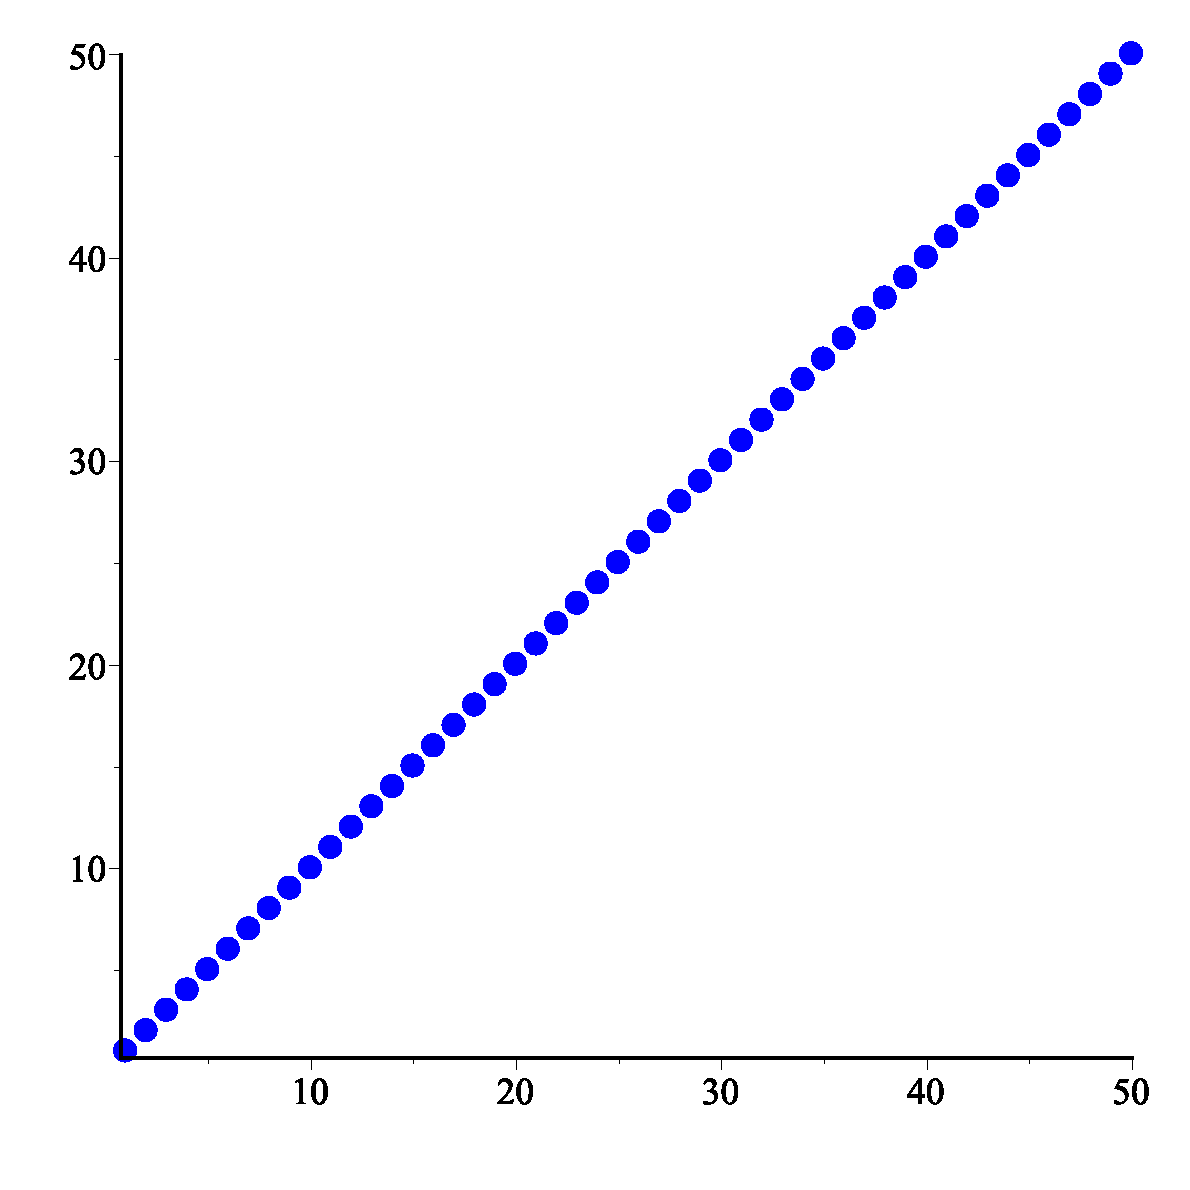
\includegraphics{figures/8_1_Sequence_n.eps}} 
%\end{center}
We recalling that a function $f$ has a limit $L$ at infinity if we can make the values of $f(x)$ as large as we want by choosing $x$ as large as we need. Since we can make the values of $n$ in our sequence as large as we want by choosing $n$ to be as large as we need, we suspect that this sequence does not have a limit as $n$ goes to infinity.

\item By observation we see that a formula for $s_n$ is $s_n = \frac{1}{n}$. A plot of the first 50 points in the sequence is shown here.
%\begin{center} \resizebox{!}{1.75in}{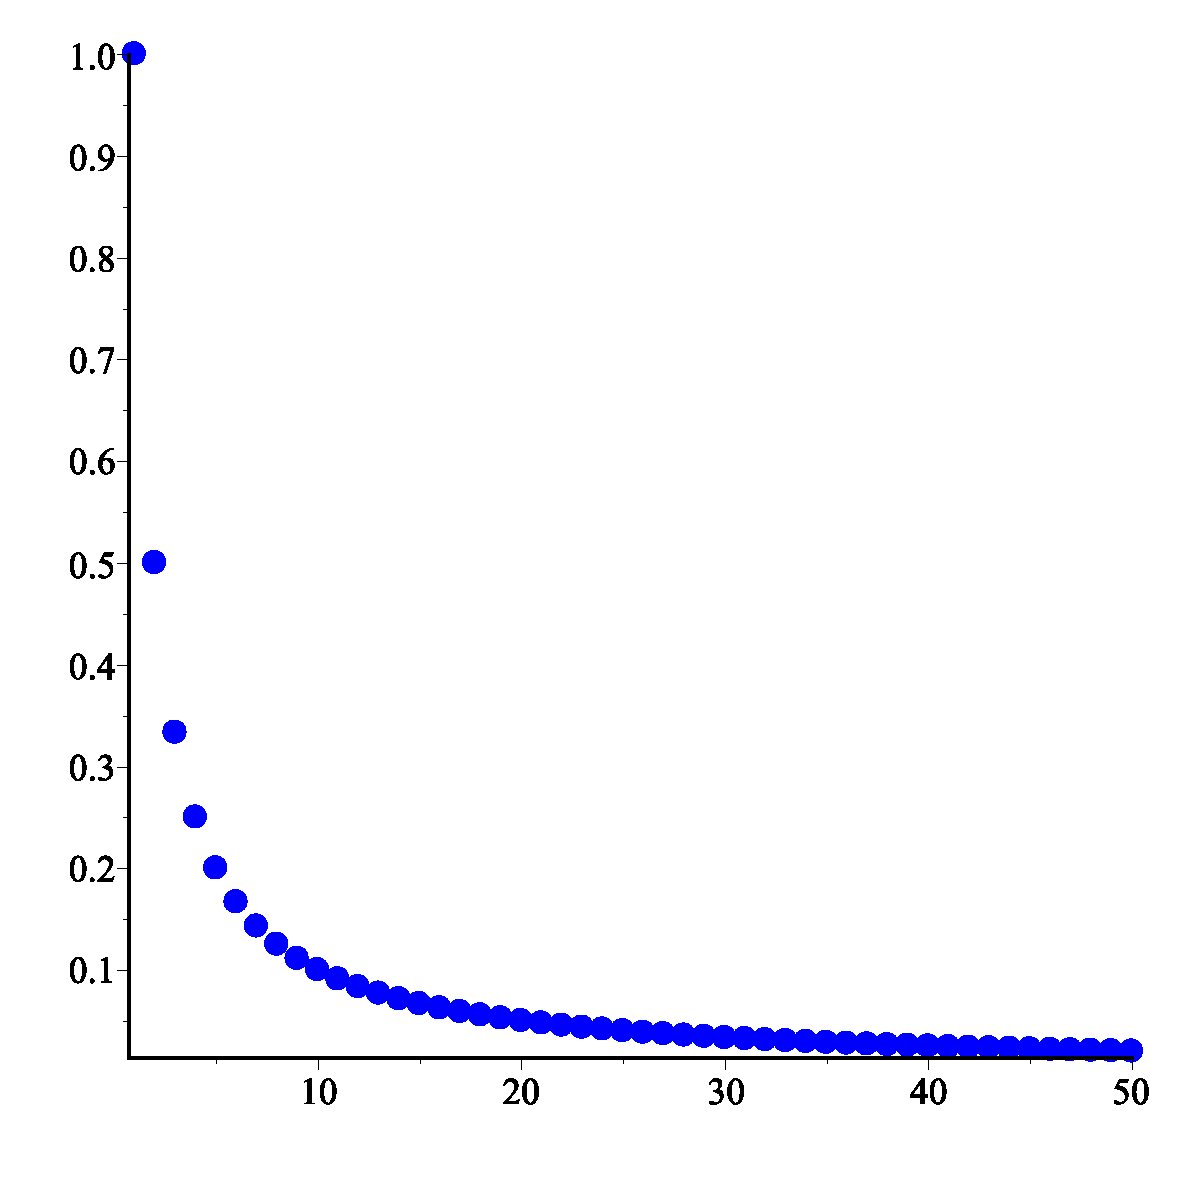
\includegraphics{figures/8_1_Sequence_1overn.eps}} \end{center}
Since we can make the values of $\frac{1}{n}$ in our sequence as close to 0 as we want by choosing $n$ to be as large as we need, we suspect that this sequence has a limit of 0 as $n$ goes to infinity.

\item Since the numerator is always 1 more than the denominator, a formula for $s_n$ is $s_n = \frac{n+1}{n}$. A plot of the first 50 points in the sequence is shown here.
%\begin{center} \resizebox{!}{1.75in}{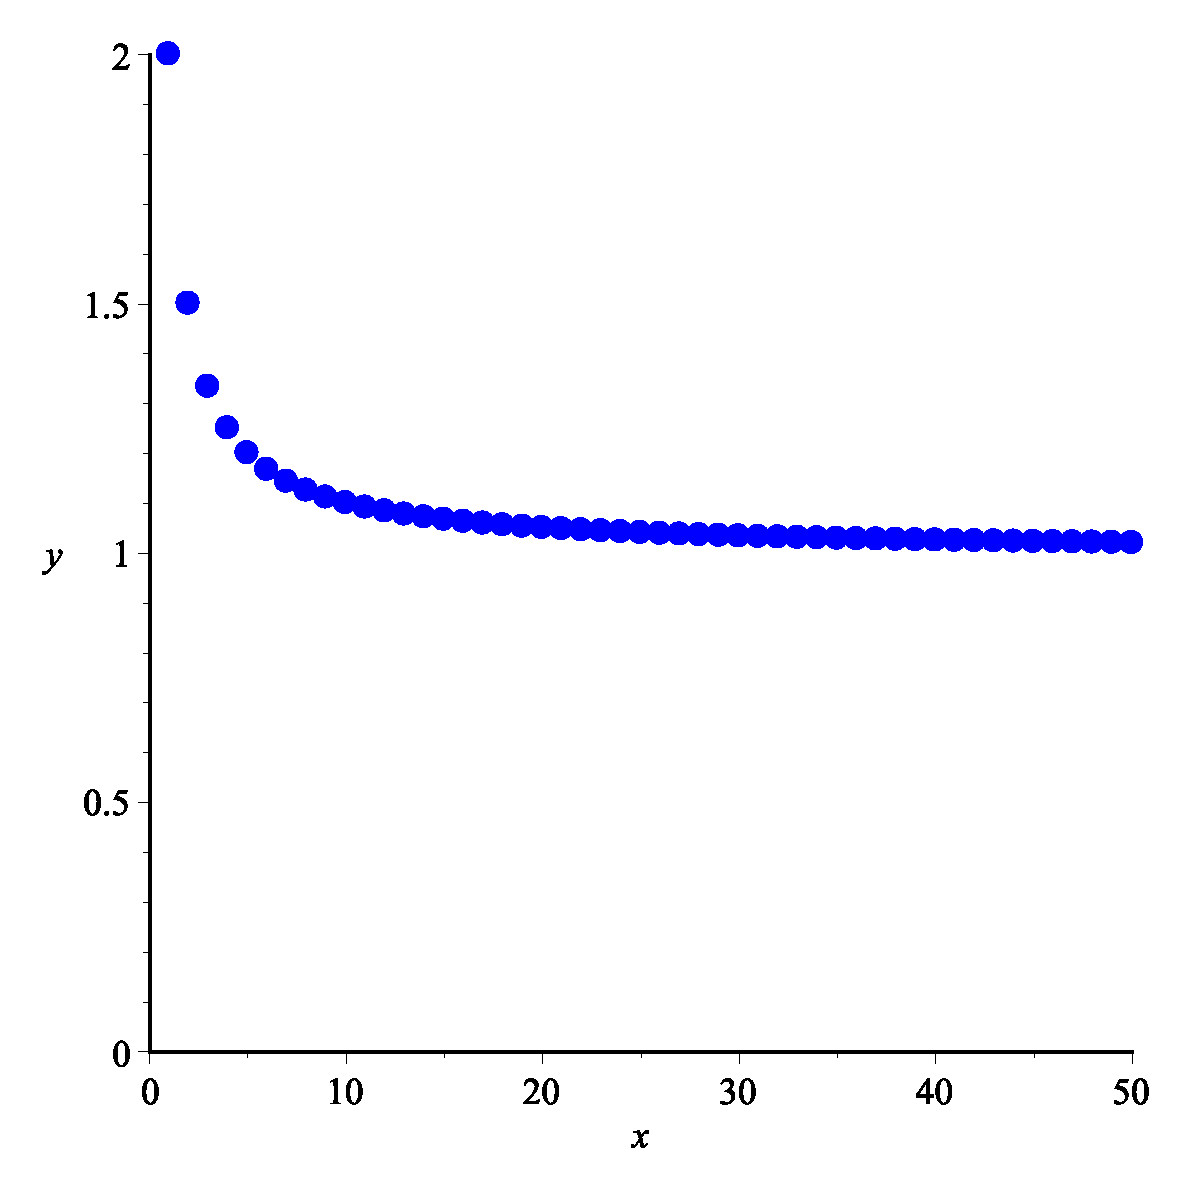
\includegraphics{figures/8_1_Sequence_nplus1overn.eps}} \end{center}
Since we can make the values of $\frac{n+1}{n}$ in our sequence as close to 1 as we want by choosing $n$ to be as large as we need, we suspect that this sequence has a limit of 1 as $n$ goes to infinity.

\ea
\end{activitySolution}
\aftera  % ACTIVITY

Next we formalize the ideas from Activity~\ref{7.1.Act1}.

\begin{activity} \label{7.1.Act2}
\ba
\item State clearly what it means for a continuous function $f$ to have a limit $L$ as $x \to \infty$.

\item Given that an infinite sequence of real numbers is a function from the integers to the real numbers, apply the idea from part (a) to explain what you think it means for a sequence $\{s_n\}$ to have a limit as $n \to \infty$.  

\item Based on your response to (b), decide if the sequence $\left\{ \frac{1+n}{2+n}\right\}$ has a limit as $n \to \infty$. If so, what is the limit? If not, why not?

\ea
\end{activity}

\begin{smallhint}
\ba
	\item Small hints for each of the prompts above.
\ea
\end{smallhint}
\begin{bighint}
\ba
	\item Big hints for each of the prompts above.
\ea
\end{bighint}
\begin{activitySolution}
\ba
	\item A continuous function $f$ has a limit $L$ as the independent variable $x$ goes to infinity if we can make the values of $f(x)$ as close to $L$ as we want by choosing $x$ as large as we need. 
    \item We expect that a sequence $\{s_n\}$ will have a limit $L$ as $n$ goes to infinity if we can make the entries $s_n$ in the sequence as close to $L$ as we want by choosing $n$ as large as we need.
    \item As $n$ gets large, the constant terms become infinitesimally small compared to $n$ and so $\frac{1+n}{2+n}$ looks like $\frac{n}{n}$ or 1 for large $n$. So the sequence $\left\{ \frac{1+n}{2+n}\right\}$ has a limit of 1 at infinity.   
\ea
\end{activitySolution}
\aftera  % ACTIVITY

\begin{marginfigure}[4cm] % MARGIN FIGURE
\subfloat[]{\margingraphics{figures/figseq1a}}

\subfloat[]{\margingraphics{figures/figseq1b}}

\subfloat[]{\margingraphics{figures/figseq1c}}
\caption{Plotting sequences from Example~\ref{eg:7.1.1}.} \label{F:eg:7.1.1}
\end{marginfigure}

\begin{example} \label{eg:7.1.1} % EXAMPLE
List the first four terms of the following sequences.

\begin{enumerate}[1), leftmargin=*]
\item $\ds \{a_n\} = \left\{\frac{3^n}{n!}\right\}$
\item $\{a_n\} = \{4+(-1)^n\}$
\item $\ds \{a_n\} = \left\{\frac{(-1)^{n(n+1)/2}}{n^2}\right\}$
\end{enumerate}

\solution
\begin{enumerate}[1)]
\item	 $\ds a_1=\frac{3^1}{1!} = 3$; $\ds a_2= \frac{3^2}{2!} = \frac92$; $\ds a_3 = \frac{3^3}{3!} = \frac92$; $\ds a_4 = \frac{3^4}{4!} = \frac{27}8$

We can plot the terms of a sequence with a scatter plot. The ``$x$''-axis is used for the values of $n$, and the values of the terms are plotted on the $y$-axis. To visualize this sequence, see Figure~\ref{F:eg:7.1.1}-(a).\\

\item		$a_1= 4+(-1)^1 = 3$;\qquad $a_2 = 4+(-1)^2 = 5$; 

\noindent $a_3=4+(-1)^3 = 3$; \qquad $a_4 = 4+(-1)^4 = 5$. Note that the range of this sequence is finite, consisting of only the values 3 and 5. This sequence is plotted in Figure \ref{F:eg:7.1.1}-(b).\\

\item		$\ds a_1= \frac{(-1)^{1(2)/2}}{1^2} = -1$; \qquad $\ds a_2 = \frac{(-1)^{2(3)/2}}{2^2} =-\frac14$

\noindent $\ds a_3 = \frac{(-1)^{3(4)/2}}{3^2} = \frac19$ \qquad $\ds a_4 = \frac{(-1)^{4(5)/2}}{4^2} = \frac1{16}$; 

\noindent $\ds a_5 = \frac{(-1)^{5(6)/2}}{5^2}=-\frac1{25}$.

\noindent We gave one extra term to begin to show the pattern of signs is ``$-$, $-$, $+$, $+$, $-$, $-$, $\ldots$, due to the fact that the exponent of $-1$ is a special quadratic. This sequence is plotted in Figure \ref{F:eg:7.1.1}-(c).
\end{enumerate}
\end{example}

\begin{example} \label{eg:7.1.2} % EXAMPLE
Find the $n^\text{th}$ term of the following sequences, i.e., find a function that describes each of the given sequences.

\begin{enumerate}[1)]
\item $2, 5, 8, 11, 14, \ldots$
\item $2, -5, 10, -17, 26, -37, \ldots$
\item $1, 1, 2, 6, 24, 120, 720, \ldots$
\item $\ds \frac52, \frac52, \frac{15}8, \frac54, \frac{25}{32}, \ldots$
\end{enumerate}

\solution We should first note that there is never exactly one function that describes a finite set of numbers as a sequence. There are many sequences that start with $2$, then $5$, as our first example does. We are looking for a simple formula that describes the terms given, knowing there is possibly more than one answer.
\begin{enumerate}[1)]
\item		Note how each term is $3$ more than the previous one. This implies a linear function would be appropriate: $a(n) = a_n = 3n + b$ for some appropriate value of $b$. As we want $a_1=2$, we set $b=-1$. Thus $a_n = 3n-1$.

\item		First notice how the sign changes from term to term. This is most commonly accomplished by multiplying the terms by either $(-1)^n$ or $(-1)^{n+1}$. Using $(-1)^n$ multiplies the odd terms by $(-1)$; using $(-1)^{n+1}$ multiplies the even terms by $(-1)$. As this sequence has negative even terms, we will multiply by $(-1)^{n+1}$. 

After this, we might feel a bit stuck as to how to proceed. At this point, we are just looking for a pattern of some sort: what do the numbers $2$, $5$, $10$, $17$, etc., have in common? There are many correct answers, but the one that we'll use here is that each is one more than a perfect square. That is, $2=1^1+1$, $5=2^2+1$, $10=3^2+1$, etc. Thus our formula is $a_n= (-1)^{n+1}(n^2+1)$.

\item		One who is familiar with the factorial function will readily recognize these numbers. They are $0!$, $1!$, $2!$, $3!$, etc. Since our sequences start with $n=1$, we cannot write $a_n = n!$, for this misses the $0!$ term. Instead, we shift by $1$, and write $a_n = (n-1)!$.

\item		This one may appear difficult, especially as the first two terms are the same, but a little ``sleuthing'' will help. Notice how the terms in the numerator are always multiples of $5$, and the terms in the denominator are always powers of $2$. Does something as simple as $a_n = \frac{5n}{2^n}$ work?

When $n=1$, we see that we indeed get $5/2$ as desired. When $n=2$, we get $10/4 = 5/2$. Further checking shows that this formula indeed matches the other terms of the sequence.
\end{enumerate}
\end{example}

A common mathematical endeavor is to create a new mathematical object (for instance, a sequence) and then apply previously known mathematics to the new object. We do so here. The fundamental concept of calculus is the limit, so we will investigate what it means to find the limit of a sequence.

\definition{Limit of a Sequence, Convergent, Divergent} %DEFINITION
{Let $\{a_n\}$ be a sequence and let $L$ be a real number. Given any $\epsilon>0$, if an $m$ can be found such that $|a_n-L|<\epsilon$ for all $n>m$, then we say the \textbf{limit of $\{a_n\}$, as $n$ approaches infinity, is $L$}, denoted $$\lim_{n\to\infty}a_n = L.$$

If $\ds\lim_{n\to\infty} a_n$ exists, we say the sequence \emph{converges}; otherwise, the sequence \emph{diverges}.\index{limit!of sequence}\index{sequences!limit}\index{convergence!of sequence}\index{divergence!of sequence}\index{sequences!convergent}\index{sequences!divergent}
} %end DEFINITION

This definition states, informally, that if the limit of a sequence is $L$, then if you go far enough out along the sequence, all subsequent terms will be \emph{really close} to $L$. Of course, the terms ``far enough'' and ``really close'' are subjective terms, but hopefully the intent is clear.

This definition is reminiscent of the $\epsilon$--$\delta$ proofs of Chapter~\ref{CH:1}. In that chapter we developed other tools to evaluate limits apart from the formal definition; we do so here as well.

\concept{Limit of a Sequence}  %concept
{Let $\{a_n\}$ be a sequence and let $f(x)$ be a function where $f(n) = a_n$ for all $n$ in $\mathbb{N}$. 
\begin{enumerate}
\item		If $\ds \lim_{x\to\infty} f(x) = L$, then $\ds\lim_{n\to\infty} a_n = L$.
\item		If $\ds \lim_{x\to\infty} f(x)$ does not exist, then $\{a_n\}$ diverges.
\end{enumerate}
} %end concept

When we considered limits before, the domain of the function was an interval of real numbers. Now, as we consider limits, the domain is restricted to $\mathbb{N}$, the natural numbers; this restriction of the domain does not affect the outcome of the limit and whatever tools we developed in Chapter~\ref{CH:1} to evaluate limits can be applied here as well.

\begin{example} \label{eg:7.1.3} % EXAMPLE
Determine the convergence or divergence of the following sequences.

\begin{enumerate}[1)]
\item $\ds\{a_n\} = \left\{\frac{3n^2-2n+1}{n^2-1000}\right\}$
\item $\{a_n\} = \{\cos n \}$
\item  $\ds\{a_n\} = \left\{\frac{(-1)^n}{n}\right\}$
\end{enumerate}

\solution
\begin{enumerate}[1)]
\item We can state that $\ds\lim_{x\to\infty} \frac{3x^2-2x+1}{x^2-1000} = 3$. (We could have also directly applied l'H\^opital's Rule.) Thus the sequence $\{a_n\}$ converges, and its limit is $3$. A scatter plot of every $5$ values of $a_n$ is given in Figure \ref{fig:eg:7.1.3}-(a). The values of $a_n$ vary widely near $n=30$, ranging from about $-73$ to $125$, but as $n$ grows, the values approach $3$.

\item The limit $\ds\lim_{x\to\infty}\cos x$ does not exist, as the function oscillates (and takes on every value in $[-1,1]$ infinitely many times). Thus we conclude that the sequence $\{\cos n\}$ diverges. (And in this particular case, since the domain is restricted to $\mathbb{N}$, no value of $\cos n$ is repeated!) This sequence is plotted in Figure \ref{fig:eg:7.1.3}-(b); because only discrete values of cosine are plotted, it does not bear strong resemblance to the familiar cosine wave.

\item The function $f(x) = (-1)^x/x$ is not well defined. (What does $(-1)^{\sqrt{2}}$ mean? In actuality, there is an answer, but it involves \emph{complex analysis}, beyond the scope of this text.) So for now we say that we cannot determine the limit. (But we will be able to very soon.) By looking at the plot in Figure \ref{fig:eg:7.1.3}-(c), we would like to conclude that the sequence converges to $0$. That is true, but at this point we are unable to decisively say so.
\end{enumerate}
\end{example}

\begin{marginfigure}[-4CM] % MARGIN FIGURE
\subfloat[]{\margingraphics{figures/figseq4a}}

\subfloat[]{\margingraphics{figures/figseq4b}}

\subfloat[]{\margingraphics{figures/figseq4c}}
\caption{Scatter plots of the sequences in Example \ref{eg:7.1.3}.}\label{fig:eg:7.1.3}
\end{marginfigure}

\begin{activity} \label{7.1.Act3} Use graphical and/or algebraic methods to determine whether each of the following sequences converges or diverges.
\ba
\item $\ds \left\{\frac{1+2n}{3n-2}\right\}$


\item $\ds \left\{\frac{5+3^n}{10+2^n}\right\}$

\item $\ds \left\{\frac{10^n}{n!}\right\}$ (where $!$ is the \emph{factorial} symbol and $n! = n(n-1)(n-2) \cdots (2)(1)$ for any positive integer $n$ (as convention we define $0!$ to be 1)).

\ea
\end{activity}

\begin{smallhint}
\ba
	\item Small hints for each of the prompts above.
\ea
\end{smallhint}
\begin{bighint}
\ba
	\item Big hints for each of the prompts above.
\ea
\end{bighint}
\begin{activitySolution}
\ba
	\item A plot of the first 50 terms of the sequence $\left\{\frac{1+2n}{3n-2}\right\}$ is shown here.
\begin{center} \resizebox{!}{1.75in}{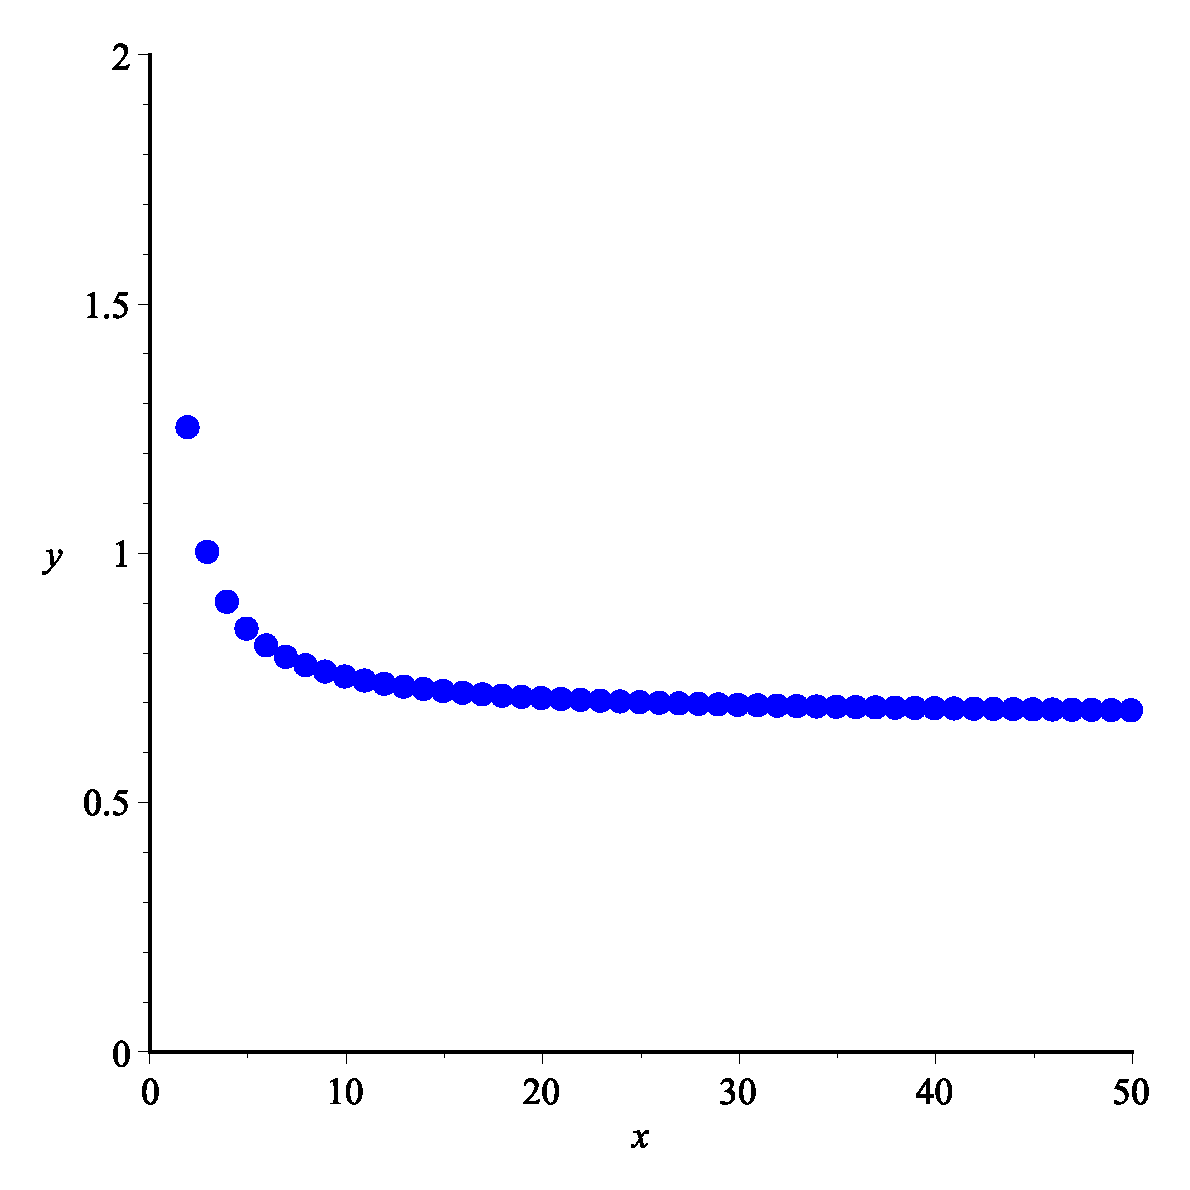
\includegraphics{figures/8_2_Sequence_a.eps}} \end{center}
The plot implies that the sequence has a limit between 0.5 and 1. For large $n$ the $2n$ term dominates the numerator and the $3n$ term the denominator. So $\frac{1+2n}{3n-2}$ looks like $\frac{2n}{3n} = \frac{2}{3}$ when $n$ is big. So the sequence $\left\{\frac{1+2n}{3n-2}\right\}$ converges to $\frac{2}{3}$.
    \item A plot of the first 50 terms of the sequence $\left\{\frac{5+3^n}{10+2^n}\right\}$ is shown here.
\begin{center} \resizebox{!}{1.75in}{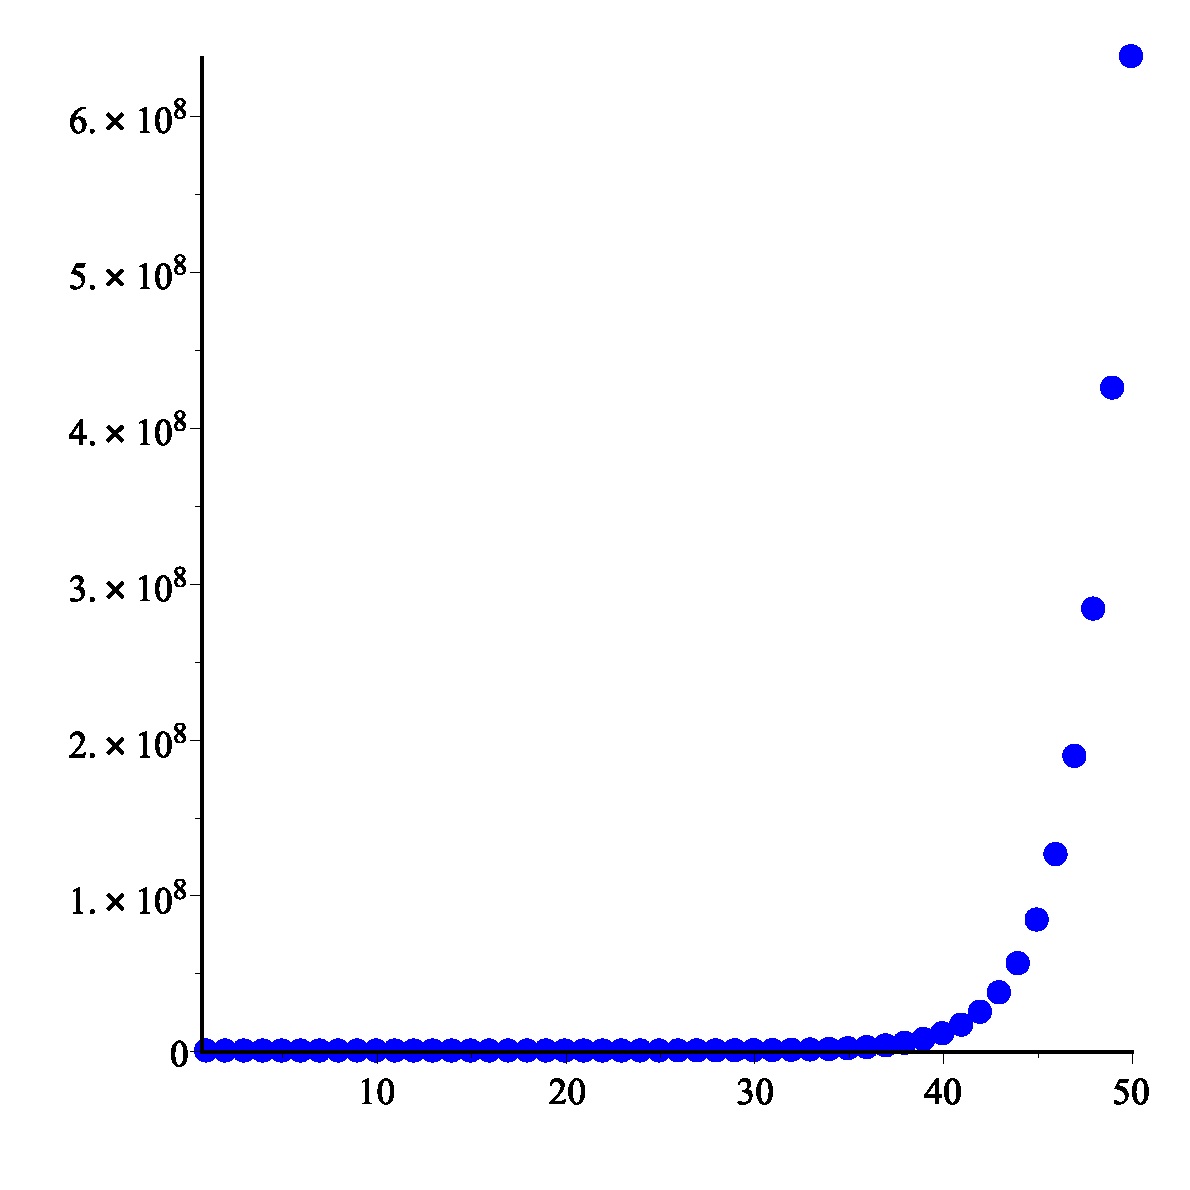
\includegraphics{figures/8_2_Sequence_b.eps}} \end{center}
The plot implies that the sequence does not have a limit as $n$ goes to infinity. For large $n$ the $3^n$ term dominates the numerator and the $2^n$ term the denominator. So $\frac{5+3^n}{10+2^n}$ looks like $\frac{3^n}{2^n} = \left(\frac{3}{2}\right)^n$ when $n$ is big. Since $\frac{3}{2} > 1$, the sequence $\left\{\frac{5+3^n}{10+2^n}\right\}$ diverges to infinity.
    \item A plot of the first 50 terms of the sequence $\left\{\frac{10^n}{n!}\right\}$ is shown here.
\begin{center} \resizebox{!}{1.75in}{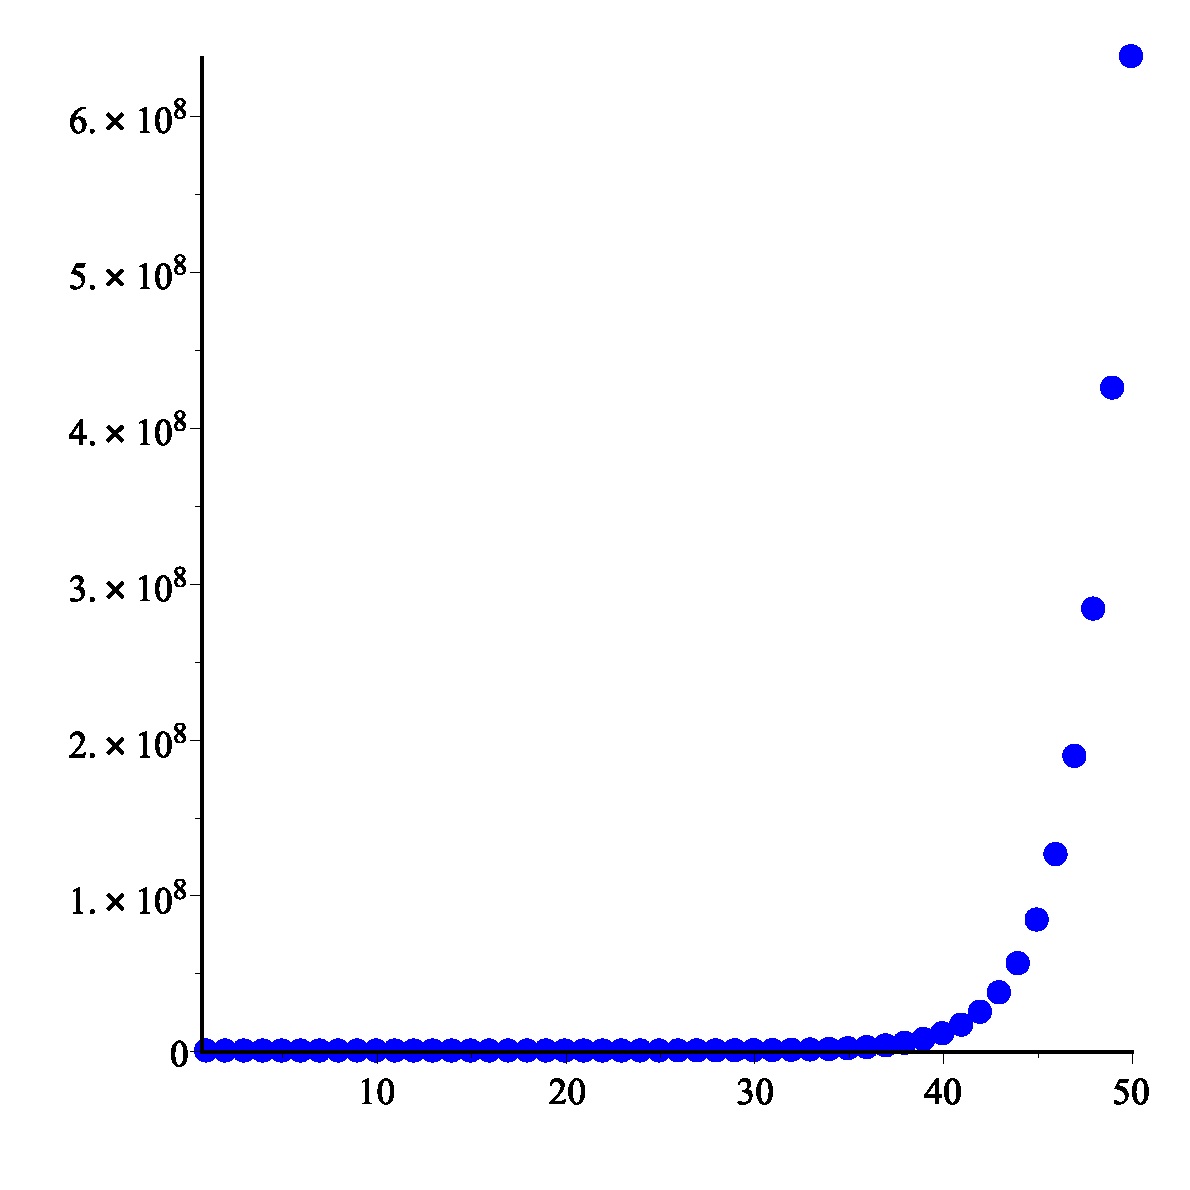
\includegraphics{figures/8_2_Sequence_b.eps}} \end{center}
Initially, it looks as though the terms increase without bound, but beginning at about $n=10$ the factorial in the denominator dominates the numerator. Notice that
 \[\frac{10^n}{n!} = \frac{10 \times 10 \times 10 \times \cdots \times 10}{1 \times 2 \times 3 \times \cdots n}\]
When $n > 20$, we have that $\frac{10}{n} < \frac{1}{2}$ and 
\begin{align*}
\frac{10^n}{n!} &= \left(\frac{10 \times 10 \times 10 \times \cdots \times 10}{1 \times 2 \times 3 \times \cdots 20}\right) \left(\frac{10 \times 10 \times 10 \times \cdots \times 10}{21 \times 22 \times 23 \times \cdots n}\right) \\
    &= \left(\frac{10^{20}}{20!}\right) \left(\frac{10}{21}\right) \left(\frac{10}{22}\right) \cdots \left(\frac{10}{n}\right)  \\
    &< \left(\frac{10^{20}}{20!}\right) \left(\frac{1}{2}\right)^{n-20}.
\end{align*}
Since $\frac{1}{2}<1$, the term $\left(\frac{1}{2}\right)^{n-20}$ goes to 0 as $n$ goes to infinity. The fact that $\frac{10^{20}}{20!}$ is a constant means that $\frac{10^n}{n!} \to 0$ as $n \to \infty$. 

\ea
\end{activitySolution}
\aftera  % ACTIVITY

It seems very clear that a sequence such as $\ds \left\{\frac{(-1)^n}{n}\right\}$ converges to 0 but we lack the formal tool to prove it. The following theorem gives us that tool.

\concept{Absolute Value Theorem} %concept
{Let $\{a_n\}$ be a sequence. If $\ds \lim_{n\to\infty} |a_n| = 0$, then $\ds \lim_{n\to\infty} a_n = 0$\index{Absolute Value Theorem}\index{limit!Absolute Value Theorem}\index{sequence!Absolute Value Theorem}
} % end concept

\begin{example} \label{eg:7.1.4} % EXAMPLE
Let the following sequences, and their limits, be given:

\begin{itemize}
\item $\ds \{a_n\} = \left\{\frac{n+1}{n^2}\right\}$, and $\ds \lim_{n\to\infty} a_n = 0$;
\item $\ds \{b_n\} = \left\{\left(1+\frac1n\right)^{n}\right\}$, and $\ds \lim_{n\to\infty} b_n = e$; and
\item $\ds \{c_n\} = \big\{n\cdot \sin (5/n)\big\}$, and $\ds \lim_{n\to\infty} c_n = 5$.
\end{itemize}

Evaluate the following limits.

\begin{enumerate}[1)]
\item $\ds \lim_{n\to\infty} (a_n+b_n)$ 
\item $\ds \lim_{n\to\infty} (b_n\cdot c_n)$ 
\item $\ds \lim_{n\to\infty} (1000\cdot a_n)$
\end{enumerate}

\solution
\begin{enumerate}[1)] 
\item Since $\ds \lim_{n\to\infty} a_n = 0$ and $\ds \lim_{n\to\infty} b_n = e$, we conclude that $\ds \lim_{n\to\infty} (a_n+b_n) = 0+e = e.$ So even though we are adding something to each term of the sequence $b_n$, we are adding something so small that the final limit is the same as before.

\item Since $\ds \lim_{n\to\infty} b_n = e$ and $\ds \lim_{n\to\infty} c_n = 5$, we conclude that $\ds \lim_{n\to\infty} (b_n\cdot c_n) = e\cdot 5 = 5e.$

\item Since $\ds \lim_{n\to\infty} a_n = 0$, we have $\ds \lim_{n\to\infty} 1000a_n =1000\cdot 0 = 0$. It does not matter that we multiply each term by $1000$; the sequence still approaches $0$. (It just takes longer to get close to $0$.)
\end{enumerate}
\end{example}

%-------------------------------
% SUBSECTION SEQUENCES PROPERTIES
%-------------------------------
\subsection*{Properties of Sequences} %\index{sequence}

We continue our study of the limits of sequences by considering some of the properties of these limits.

\concept{Properties of the Limits of Sequences} %concept
{Let $\{a_n\}$ and $\{b_n\}$ be sequences such that $\ds \lim_{n\to\infty} a_n = L$, $\ds \lim_{n\to\infty} b_n = K$, and let $c$ be a real number.

\begin{minipage}[t]{.5\linewidth}
\begin{enumerate}
\item		$\ds \lim_{n\to\infty} (a_n\pm b_n) = L\pm K$
\index{sequences!limit properties}
\item		$\ds \lim_{n\to\infty} (a_n\cdot b_n) = L\cdot K$
\end{enumerate}
\end{minipage}
\begin{minipage}[t]{.5\linewidth}
\begin{enumerate}\addtocounter{enumi}{2}
\item		$\ds \lim_{n\to\infty} (a_n/b_n) = L/K$, $K\neq 0$
\item		$\ds \lim_{n\to\infty} c\cdot a_n = c\cdot L$
\end{enumerate}
\end{minipage}
} %end concept


\begin{example} \label{eg:7.1.5} % EXAMPLE
Determine the boundedness of the following sequences.

\begin{enumerate}[1)]
\item $\ds\{a_n\}  = \left\{\frac1n\right\}$ 
\item $\{a_n\} = \{2^n\}$
\end{enumerate}

\solution
\begin{enumerate}[1)]
\item The terms of this sequence are always positive but are decreasing, so we have $0<a_n<2$ for all $n$. Thus this sequence is bounded. Figure \ref{fig:eg:7.1.5}-(a) illustrates this.

\item The terms of this sequence obviously grow without bound. However, it is also true that these terms are all positive, meaning $0<a_n$. Thus we can say the sequence is unbounded, but also bounded below. Figure \ref{fig:eg:7.1.5}-(b) illustrates this.
\end{enumerate}
\end{example}

\begin{marginfigure}
\subfloat[]{\margingraphics{figures/figseq3a}}

\subfloat[]{\margingraphics{figures/figseq3b}}
\caption{A plot of $\{a_n\} = \{1/n\}$ and $\{a_n\} = \{2^n\}$ from Example \ref{eg:7.1.5}.}
\label{fig:eg:7.1.5}
\end{marginfigure}

\begin{activity} \label{7.1.Act3} Use graphical and/or algebraic methods to determine whether each of the following sequences converges or diverges.
\ba
\item $\ds \left\{\frac{1+2n}{3n-2}\right\}$


\item $\ds \left\{\frac{5+3^n}{10+2^n}\right\}$

\item $\ds \left\{\frac{10^n}{n!}\right\}$ (where $!$ is the \emph{factorial} symbol and $n! = n(n-1)(n-2) \cdots (2)(1)$ for any positive integer $n$ (as convention we define $0!$ to be 1)).

\ea
\end{activity}

\begin{smallhint}
\ba
	\item Small hints for each of the prompts above.
\ea
\end{smallhint}
\begin{bighint}
\ba
	\item Big hints for each of the prompts above.
\ea
\end{bighint}
\begin{activitySolution}
\ba
	\item A plot of the first 50 terms of the sequence $\left\{\frac{1+2n}{3n-2}\right\}$ is shown here.
\begin{center} \resizebox{!}{1.75in}{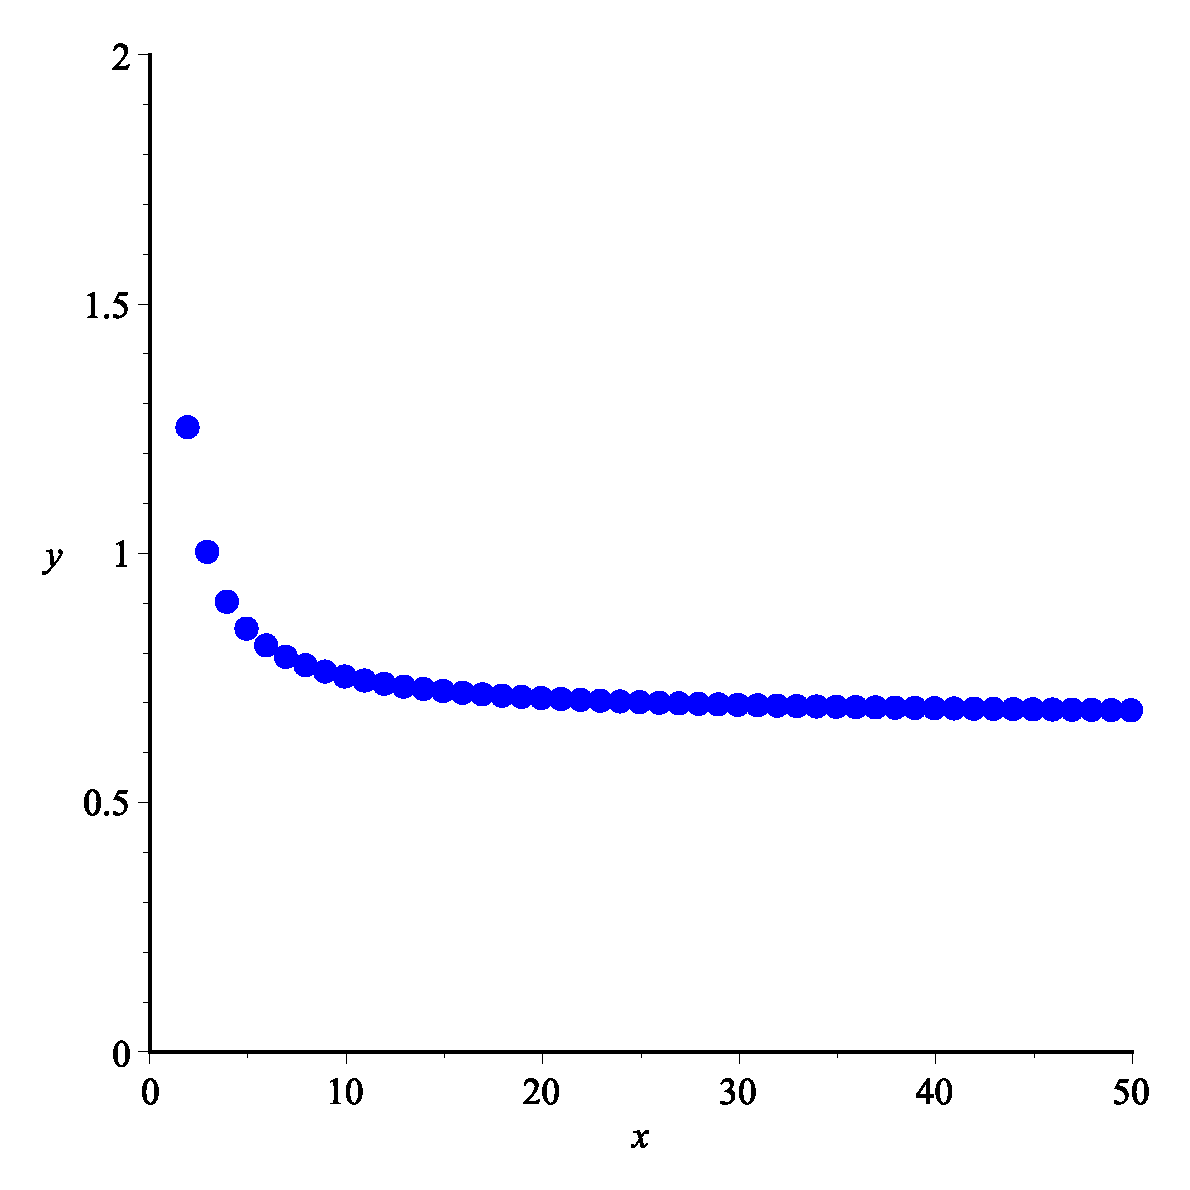
\includegraphics{figures/8_2_Sequence_a.eps}} \end{center}
The plot implies that the sequence has a limit between 0.5 and 1. For large $n$ the $2n$ term dominates the numerator and the $3n$ term the denominator. So $\frac{1+2n}{3n-2}$ looks like $\frac{2n}{3n} = \frac{2}{3}$ when $n$ is big. So the sequence $\left\{\frac{1+2n}{3n-2}\right\}$ converges to $\frac{2}{3}$.
    \item A plot of the first 50 terms of the sequence $\left\{\frac{5+3^n}{10+2^n}\right\}$ is shown here.
\begin{center} \resizebox{!}{1.75in}{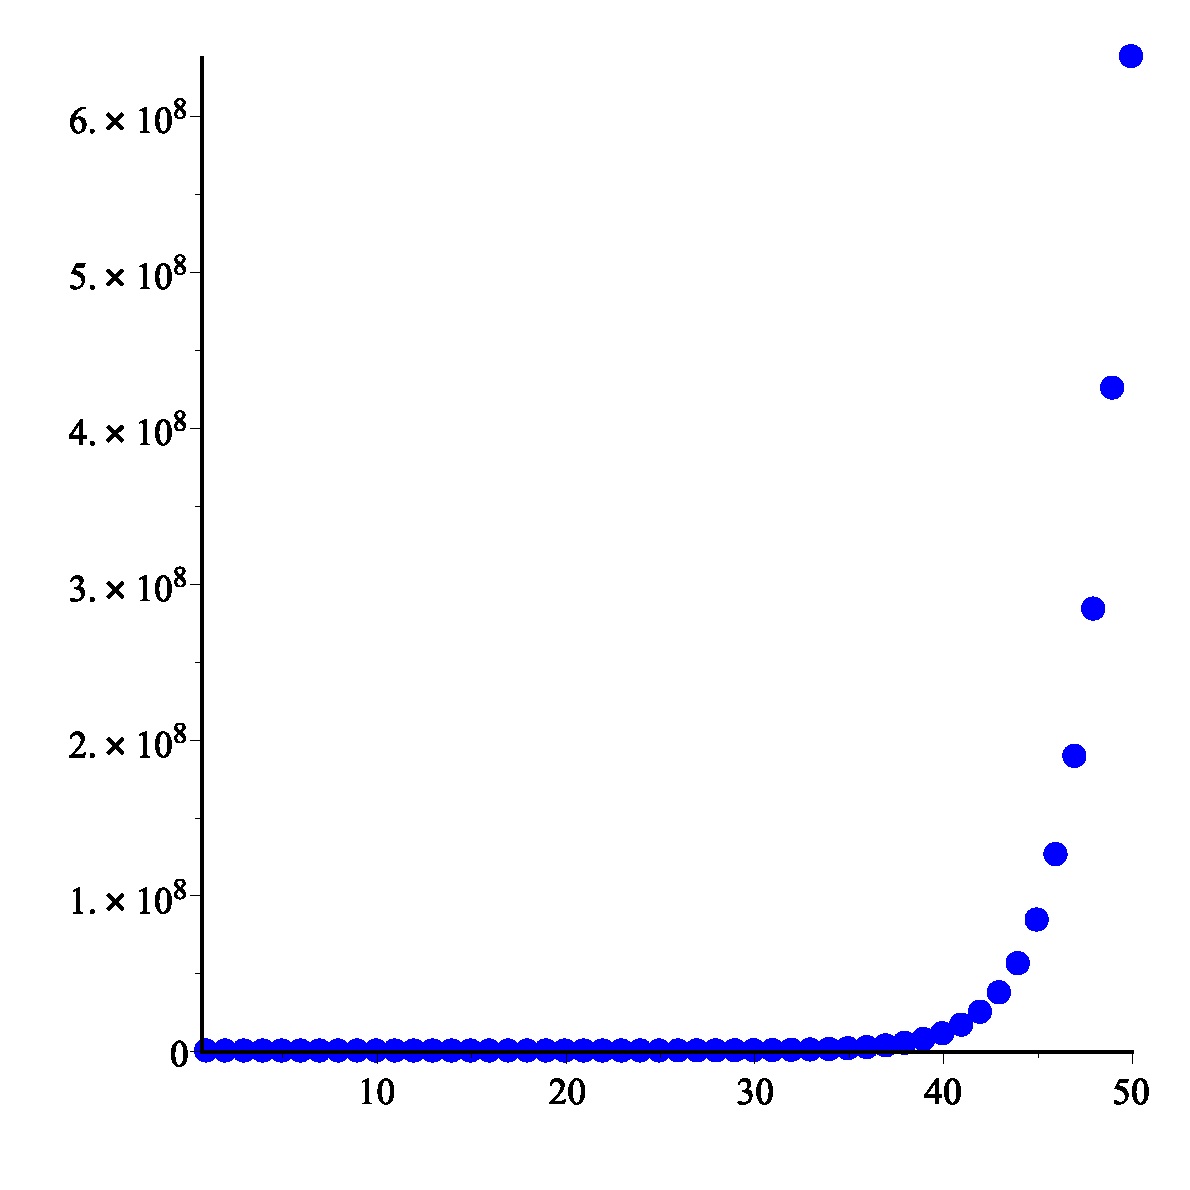
\includegraphics{figures/8_2_Sequence_b.eps}} \end{center}
The plot implies that the sequence does not have a limit as $n$ goes to infinity. For large $n$ the $3^n$ term dominates the numerator and the $2^n$ term the denominator. So $\frac{5+3^n}{10+2^n}$ looks like $\frac{3^n}{2^n} = \left(\frac{3}{2}\right)^n$ when $n$ is big. Since $\frac{3}{2} > 1$, the sequence $\left\{\frac{5+3^n}{10+2^n}\right\}$ diverges to infinity.
    \item A plot of the first 50 terms of the sequence $\left\{\frac{10^n}{n!}\right\}$ is shown here.
\begin{center} \resizebox{!}{1.75in}{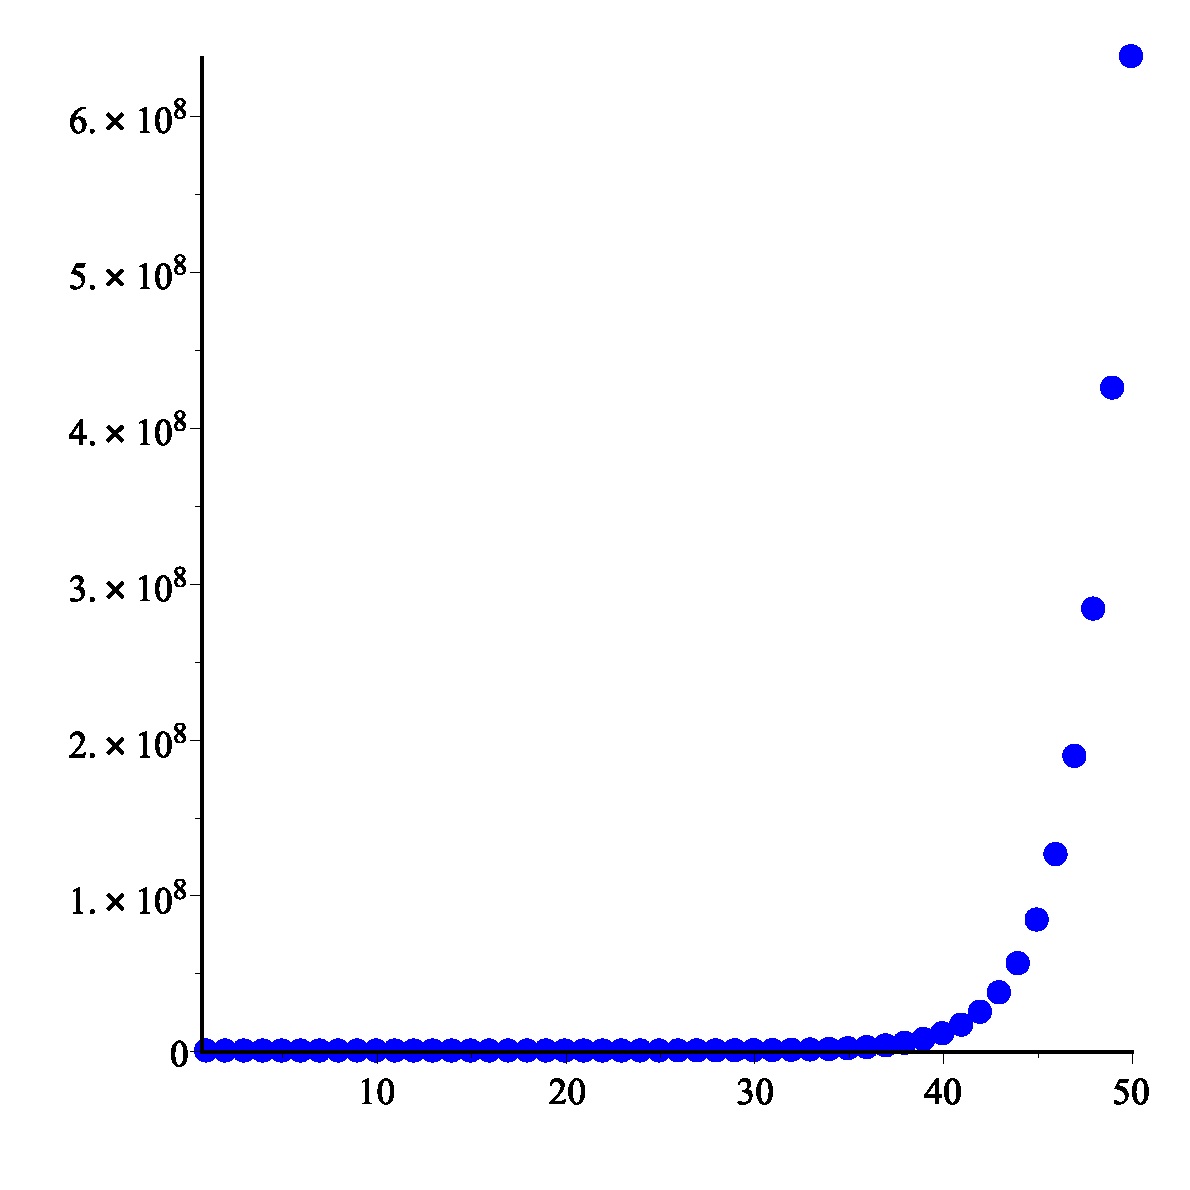
\includegraphics{figures/8_2_Sequence_b.eps}} \end{center}
Initially, it looks as though the terms increase without bound, but beginning at about $n=10$ the factorial in the denominator dominates the numerator. Notice that
 \[\frac{10^n}{n!} = \frac{10 \times 10 \times 10 \times \cdots \times 10}{1 \times 2 \times 3 \times \cdots n}\]
When $n > 20$, we have that $\frac{10}{n} < \frac{1}{2}$ and 
\begin{align*}
\frac{10^n}{n!} &= \left(\frac{10 \times 10 \times 10 \times \cdots \times 10}{1 \times 2 \times 3 \times \cdots 20}\right) \left(\frac{10 \times 10 \times 10 \times \cdots \times 10}{21 \times 22 \times 23 \times \cdots n}\right) \\
    &= \left(\frac{10^{20}}{20!}\right) \left(\frac{10}{21}\right) \left(\frac{10}{22}\right) \cdots \left(\frac{10}{n}\right)  \\
    &< \left(\frac{10^{20}}{20!}\right) \left(\frac{1}{2}\right)^{n-20}.
\end{align*}
Since $\frac{1}{2}<1$, the term $\left(\frac{1}{2}\right)^{n-20}$ goes to 0 as $n$ goes to infinity. The fact that $\frac{10^{20}}{20!}$ is a constant means that $\frac{10^n}{n!} \to 0$ as $n \to \infty$. 

\ea
\end{activitySolution}
\aftera  % ACTIVITY

%-------------------------------
% SUBSECTION MORE SEQUENCE PROPERTIES
%-------------------------------
\subsection*{More with Sequences}
There is more to learn about sequences than just their limits. We will also study their range and the relationships terms have with the terms that follow. We start with some definitions describing properties of the range.

\definition{Bounded and Unbounded Sequences} %DEFINITION
{A sequence $\{a_n\}$ is said to be \textbf{bounded} if there exists real numbers $m$ and $M$ such that $m < a_n < M$ for all $n$ in $\mathbb{N}$.\\

A sequence $\{a_n\}$ is said to be \textbf{unbounded} if it is not bounded.\\

A sequence $\{a_n\}$ is said to be \textbf{bounded above} if there exists an $M$ such that $a_n < M$ for all $n$ in $\mathbb{N}$; it is \textbf{bounded below} if there exists an $m$ such that $m<a_n$ for all $n$ in $\mathbb{N}$.
\index{sequences!boundedness}\index{bounded sequence}\index{unbounded sequence}
} %end DEFINITION


It follows from this definition that an unbounded sequence may be bounded above or bounded below; a sequence that is both bounded above and below is simply a bounded sequence.\\

%\mtable{.55}{Plots of sequences in Example \ref{ex_seq7}.}{fig:seq7}{%
%\begin{tabular}{c}
%\myincludegraphics{figures/figseq7a}\\
%(a)\rule[-25pt]{0pt}{10pt}\\ 
%\myincludegraphics{figures/figseq7b}\\
%(b)\rule[-25pt]{0pt}{10pt}\\ 
%\myincludegraphics{figures/figseq7c}\\
%(c)\\
%\end{tabular}
%}
%\mfigure{.6}{A plot of $\{a_n\} = \{n^2/n!\}$ in Example \ref{ex_seq7}.}{fig:seq7d}{figures/figseq7d}

\begin{marginfigure}[3cm] % MARGIN FIGURE
\subfloat[]{\margingraphics{figures/figseq7a}}

\subfloat[]{\margingraphics{figures/figseq7b}}

\subfloat[]{\margingraphics{figures/figseq7c}}
\caption{Plots of sequences in Example~\ref{eg:7.1.6}.}
\label{fig:seq7}
\end{marginfigure}

\begin{example} \label{eg:7.1.6} % EXAMPLE
Determine the monotonicity of the following sequences.

\begin{enumerate}[1)]
\item $\ds \{a_n\} = \left\{\frac{n+1}n\right\}$
\item	$\ds \{a_n\} = \left\{\frac{n^2+1}{n+1}\right\}$	
\item $\ds \{a_n\} = \left\{\frac{n^2-9}{n^2-10n+26}\right\}$
\item	$\ds \{a_n\} = \left\{\frac{n^2}{n!}\right\}$	
\end{enumerate}

\solution In each of the following, we will examine $a_{n+1}-a_n$. If $a_{n+1}-a_n >0$, we conclude that $a_n<a_{n+1}$ and hence the sequence is increasing. If $a_{n+1}-a_n<0$, we conclude that $a_n>a_{n+1}$ and the sequence is decreasing. Of course, a sequence need not be monotonic and perhaps neither of the above will apply.

We also give a scatter plot of each sequence. These are useful as they suggest a pattern of monotonicity, but analytic work should be done to confirm a graphical trend.

\begin{enumerate}[1)]
\item	
\begin{align*}
a_{n+1}-a_n &= \frac{n+2}{n+1} - \frac{n+1}{n} \\		
&= \frac{(n+2)(n)-(n+1)^2}{(n+1)n} \\
&=	\frac{-1}{n(n+1)} \\
&<0 \quad\text{ for all $n$.}
\end{align*}
				
Since $a_{n+1}-a_n<0$ for all $n$, we conclude that the sequence is decreasing.

\item	
\begin{align*}	
a_{n+1}-a_n &= \frac{(n+1)^2+1}{n+2} - \frac{n^2+1}{n+1} \\		
&= \frac{\big((n+1)^2+1\big)(n+1)- (n^2+1)(n+2)}{(n+1)(n+2)}\\
&=	\frac{n^2+4n+1}{(n+1)(n+2)} \\
&> 0 \quad \text{ for all $n$.}
\end{align*}
					
Since $a_{n+1}-a_n>0$ for all $n$, we conclude the sequence is increasing.

\item We can clearly see in Figure \ref{fig:seq7}-(c), where the sequence is plotted, that it is not monotonic. However, it does seem that after the first 4 terms it is decreasing. To understand why, perform the same analysis as done before:
\begin{align*}
a_{n+1}-a_n &= \frac{(n+1)^2-9}{(n+1)^2-10(n+1)+26} - \frac{n^2-9}{n^2-10n+26} \\		
&= \frac{n^2+2n-8}{n^2-8n+17}-\frac{n^2-9}{n^2-10n+26}\\
&= \frac{(n^2+2n-8)(n^2-10n+26)-(n^2-9)(n^2-8n+17)}{(n^2-8n+17)(n^2-10n+26)}\\
&= \frac{-10n^2+60n-55}{(n^2-8n+17)(n^2-10n+26)}.
\end{align*}

We want to know when this is greater than, or less than, $0$, therefore we are only concerned with the numerator. Using the quadratic formula, we can determine that $-10n^2+60n-55=0$ when $n\approx 1.13, 4.87$. So for $n<1.13$, the sequence is decreasing. Since we are only dealing with the natural numbers, this means that $a_1 > a_2$.

Between $1.13$ and $4.87$, i.e., for $n=2$, $3$ and $4$, we have that $a_{n+1}>a_n$ and the sequence is increasing. (That is, when $n=2$, $3$ and $4$, the numerator $-10n^2+60n+55$ from the fraction above is $>0$.)

When $n> 4.87$, i.e, for $n\geq 5$, we have that $-10n^2+60n+55<0$, hence $a_{n+1}-a_n<0$, so the sequence is decreasing.

In short, the sequence is simply not monotonic. However, it is useful to note that for $n\geq 5$, the sequence is monotonically decreasing. 

\item Again, the plot in Figure \ref{fig:seq7d} shows that the sequence is not monotonic, but it suggests that it is monotonically decreasing after the first term. We perform the usual analysis to confirm this.
\begin{align*}	
a_{n+1}-a_n &= \frac{(n+1)^2}{(n+1)!} - \frac{n^2}{n!} \\
&= \frac{(n+1)^2-n^2(n+1)}{(n+1)!} \\
&=	\frac{-n^3+2n+1}{(n+1)!}
\end{align*}
					
When $n=1$, the above expression is $>0$; for $n\geq 2$, the above expression is $<0$. Thus this sequence is not monotonic, but it is monotonically decreasing after the first term.
\end{enumerate}
\end{example}

\begin{marginfigure}[-6cm] % MARGIN FIGURE
\margingraphics{figures/figseq7d}
\caption{Plots of sequences in Example~\ref{eg:7.1.6}.}
\label{fig:seq7d}
\end{marginfigure}

The previous example produces some interesting concepts. First, we can recognize that the sequence $\ds\left\{1/n\right\}$ converges to 0. This says, informally, that ``most'' of the terms of the sequence are ``really close'' to 0. This implies that the sequence is bounded, using the following logic. First, ``most'' terms are near 0, so we could find some sort of bound on these terms, which is $\epsilon$. That leaves a ``few'' terms that are not near $0$ (i.e., a \emph{finite} number of terms). A finite list of numbers is always bounded. 

This logic implies that if a sequence converges, it must be bounded. This is indeed true, as stated by the following concept.

\concept{Convergent Sequences are Bounded} %concept
{Let $\ds \left\{a_n\right\}$ be a convergent sequence. Then $\{a_n\}$ is bounded.
\index{bounded sequence!convergence}\index{convergence!of sequence}\index{sequences!convergent}
} % end concept

\textbf{Note:} Keep in mind what the concept does \emph{not} say. It does not say that bounded sequences must converge, nor does it say that if a sequence does not converge, it is not bounded.

In Example~\ref{eg:7.1.4} we saw the sequence $\ds \{b_n\} = \left\{\left(1+1/n\right)^{n}\right\}$, where it was stated that $\ds \lim_{n\to\infty} b_n = e$.  Even though it may be difficult to intuitively grasp the behavior of this sequence, we know immediately that it is bounded.

Another interesting concept to come out of Example~\ref{eg:7.1.5} again involves the sequence $\{1/n\}$. We stated, without proof, that the terms of the sequence were decreasing. That is, that $a_{n+1} < a_n$ for all $n$. (This is easy to show. Clearly $n < n+1$. Taking reciprocals flips the inequality: $1/n > 1/(n+1)$. This is the same as $a_n > a_{n+1}$.) Sequences that either steadily increase or decrease are important, so we give this property a name.

\definition{Monotonic Sequences} %definition
{\begin{enumerate}
\item		A sequence $\{a_n\}$ is \textbf{monotonically increasing} if $a_n \leq a_{n+1}$ for all $n$, i.e.,
 $$a_1 \leq a_2 \leq a_3 \leq \cdots a_n \leq a_{n+1} \cdots$$
 \item	A sequence $\{a_n\}$ is \textbf{monotonically decreasing} if $a_n \geq a_{n+1}$ for all $n$, i.e.,
 $$a_1 \geq a_2 \geq a_3 \geq \cdots a_n \geq a_{n+1} \cdots$$
 \item	A sequence is \textbf{monotonic} if it is monotonically increasing or monotonically decreasing.
\index{sequences!monotonic}\index{monotonic sequence}
 \end{enumerate}
} %end definition

{\textbf{Note:} It is sometimes useful to call a monotonically increasing sequence \emph{strictly increasing} if $a_n < a_{n+1}$ for all $n$; i.e, we remove the possibility that subsequent terms are equal.  A similar statement holds for \emph{strictly decreasing.}


%\input{examples/7-1_Eg7.tex} %example monotonicity

Knowing that a sequence is monotonic can be useful. In particular, if we know that a sequence is bounded and monotonic, we can conclude it converges! Consider, for example, a sequence that is monotonically decreasing and is bounded below. We know the sequence is always getting smaller, but that there is a bound to how small it can become. This is enough to prove that the sequence will converge, as stated in the following theorem.

\concept{Bounded Monotonic Sequences are Convergent}%concept 
{\begin{enumerate}
\item		Let $\{a_n\}$ be a bounded, monotonic sequence. Then $\{a_n\}$ converges; i.e., $\ds \lim_{n \to\infty}a_n$ exists.
\item		Let $\{a_n\}$ be a monotonically increasing sequence that is bounded above. Then $\{a_n\}$ converges.
\item		Let $\{a_n\}$ be a monotonically decreasing sequence that is bounded below. Then $\{a_n\}$ converges.
\index{sequences!convergent}\index{convergence!of monotonic sequences}
\end{enumerate}
} %end concept

Consider once again the sequence $\{a_n\} = \{1/n\}$. It is easy to show it is monotonically decreasing and that it is always positive (i.e., bounded below by $0$). Therefore we can conclude that the sequence converges. We already knew this by other means, but in the following section this theorem will become very useful.

Sequences are a great source of mathematical inquiry. The On-Line Encyclopedia of Integer Sequences (\url{http://oeis.org}) contains thousands of sequences and their formulae. (As of this writing, there are $218,626$ sequences in the database.) Perusing this database quickly demonstrates that a single sequence can represent several different ``real life'' phenomena. 

Interesting as this is, our interest actually lies elsewhere. We are more interested in the \emph{sum} of a sequence. That is, given a sequence $\{a_n\}$, we are very interested in $a_1+a_2+a_3+\cdots$. Of course, one might immediately counter with ``Doesn't this just add up to infinity?'' Many times, yes, but there are many important cases where the answer is no. This is the topic of \emph{series}, which we begin to investigate in the next section.



%-------------
% SUMMARY
%-------------
\begin{summary}
\item A sequence is a list of objects in a specified order. We will typically work with sequences of real numbers and can also think of a sequence as a function from the positive integers to the set of real numbers.
\item A sequence $\{s_n\}$ of real numbers converges to a number $L$ if we can make every value of  $s_k$ for $k \ge n$ as close as we want to $L$ by choosing $n$ sufficiently large.
\item A sequence diverges if it does not converge.
\end{summary}

%------------------
% EXERCISES
%------------------
%\printexercises{exercises/08_01_exercises}